\documentclass[11pt,letterpaper]{article}

%%%%%%%%%%%%%%%%%%%%%%%%%%%%%%%%%%%
% IMPORTACIÓN DE CONFIGURACIONES
%%%%%%%%%%%%%%%%%%%%%%%%%%%%%%%%%%%

\input{configuracion}

%%%%%%%%%%%%%%%%%%%%%%%%%%%%
% INICIO DE DOCUMENTO
%%%%%%%%%%%%%%%%%%%%%%%%%%%%

\begin{document}

%%%%%%%%%%%%%%%%%%%%%%%%%%%%
% ENCABEZADO
%%%%%%%%%%%%%%%%%%%%%%%%%%%%
\begin{center}
    \begin{minipage}{3cm}
    	\begin{center}
    		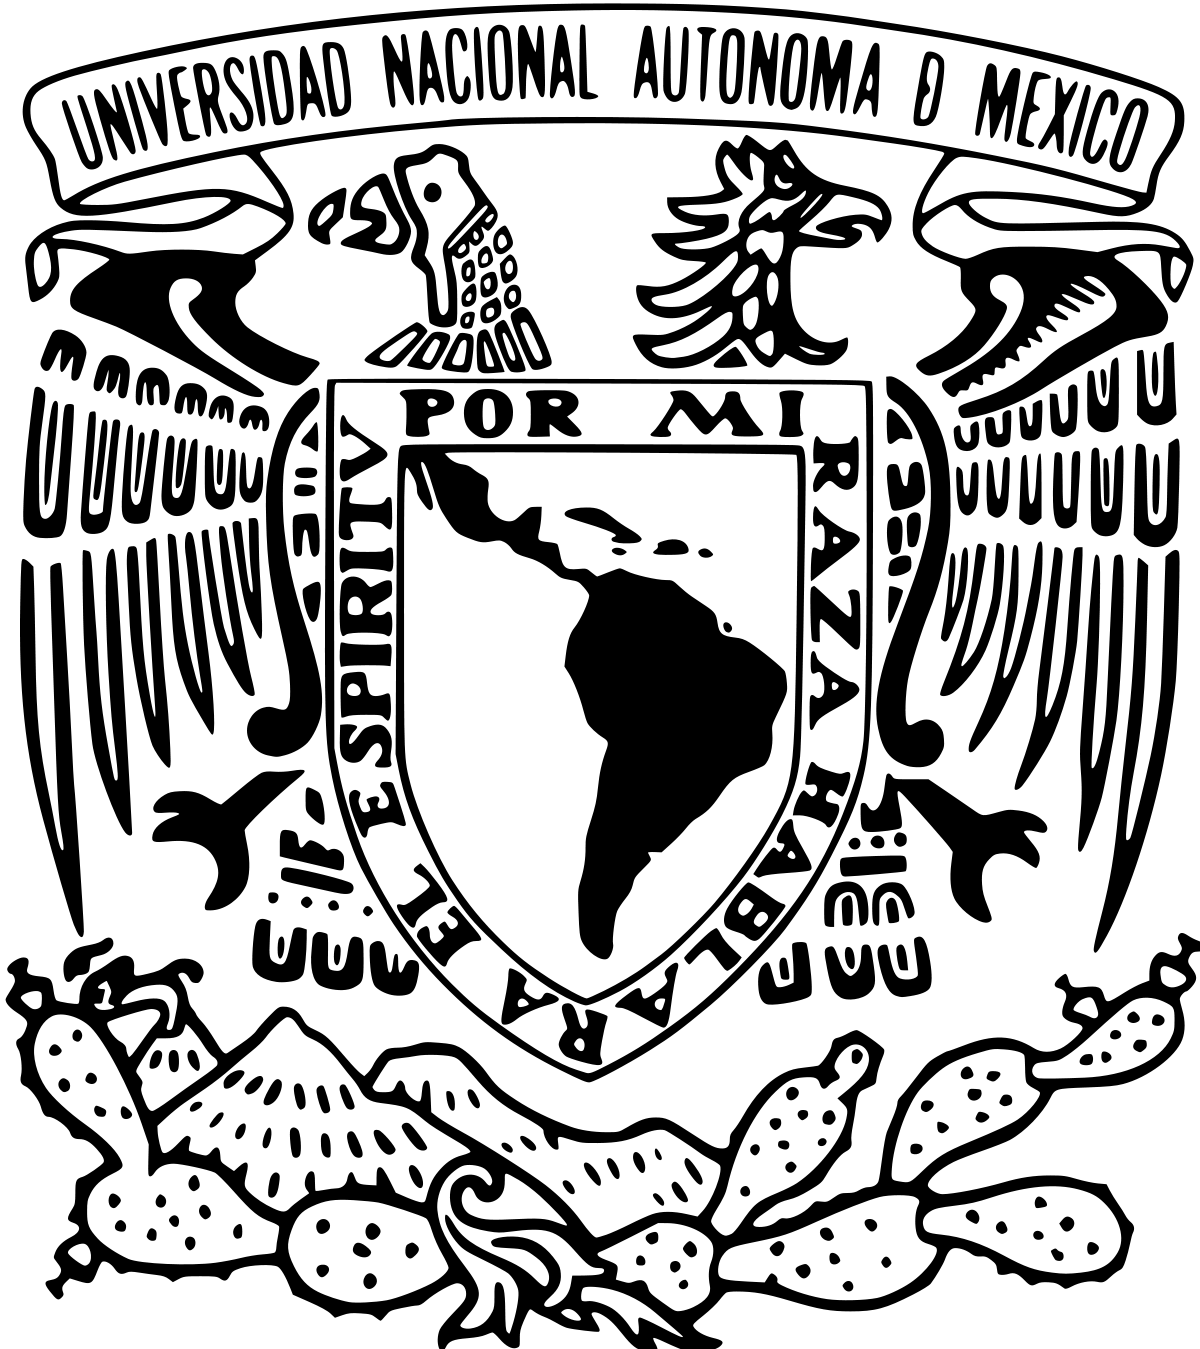
\includegraphics[height=3.4cm]{Logo_UNAM.png}
    	\end{center}
    \end{minipage}\hfill
    \begin{minipage}{10cm}
    	\begin{center}
    	\textbf{\large Universidad Nacional Autónoma de México}\\[0.1cm]
        \textbf{Facultad de Ciencias}\\[0.1cm]
        \textbf{Enlaces útiles}\\[0.1cm]
        Martínez Castro Alvaro Leonardo\\[0.1cm]
        \today
    	\end{center}
    \end{minipage}\hfill
    \begin{minipage}{3cm}
    	\begin{center}
    		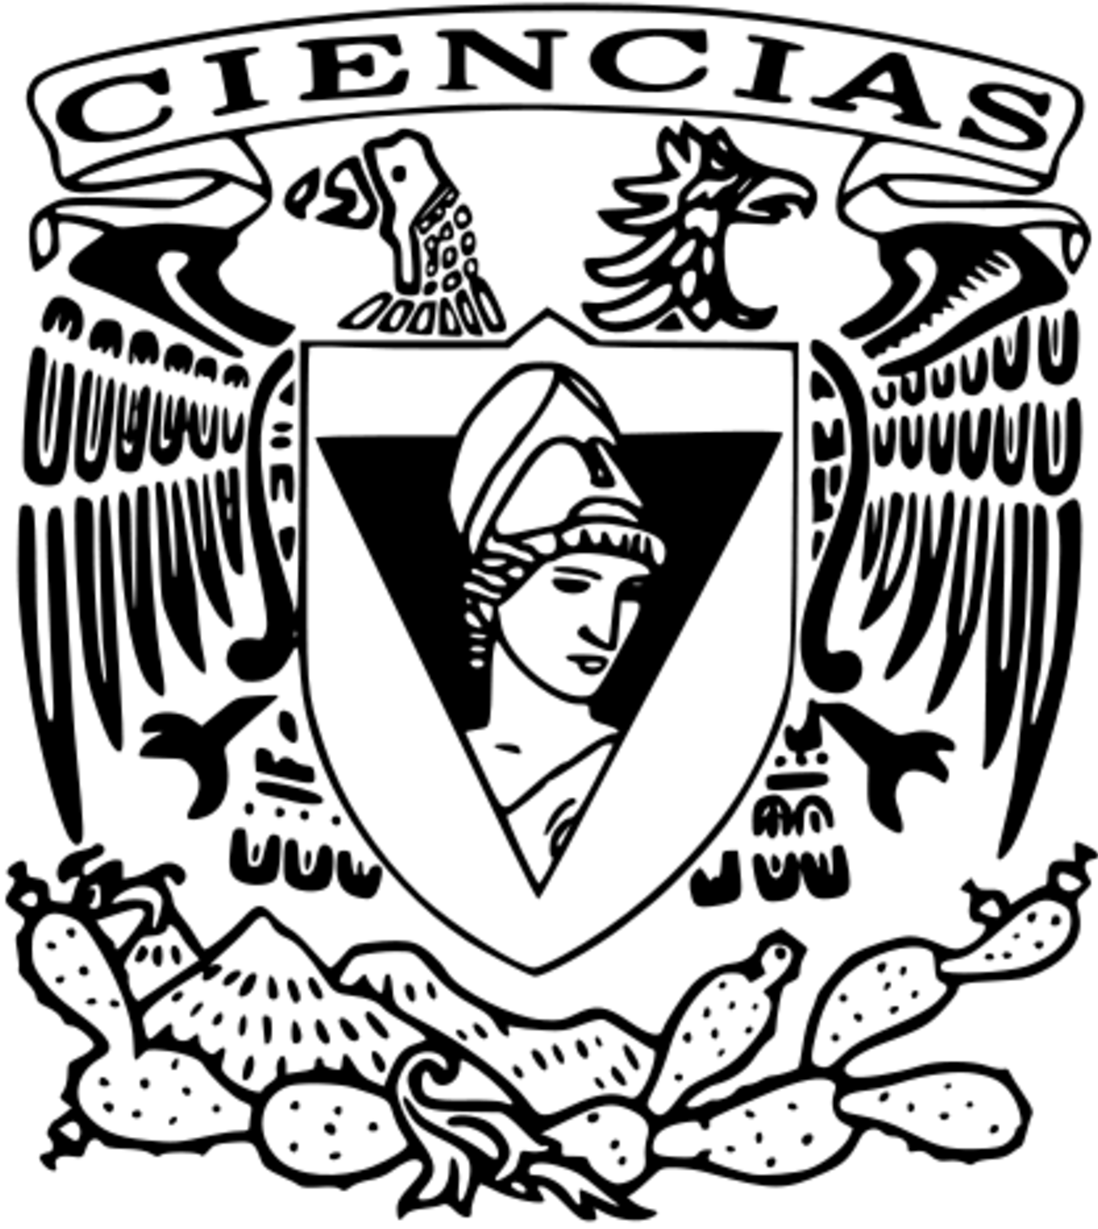
\includegraphics[height=3.4cm]{Logo_FC.png}
    	\end{center}
    \end{minipage}
\end{center}

\rule{17cm}{0.1mm}

%%%%%%%%%%%%%%%%%%%%%%%%%%%%
% FIN DE ENCABEZADO
%%%%%%%%%%%%%%%%%%%%%%%%%%%%

\begin{intro}
 Éste documento tiene algunos enlaces que pueden servir de utilidad para los estudiantes de Facultad de Ciencias, UNAM. Siéntete libre de modificar el documento y realizar los commits necesarios para añadir más recursos. 
\end{intro}

\begin{inciso}{Enlaces}
- \begin{itemize}
    \item \textbf{El blog de Leo:} https://blog.nekomath.com
    \item \textbf{ReefSeek:} https://www.refseek.com
    \item \textbf{DeepSeek:} https://www.deepseek.com
    \item \textbf{BidiUnam:} https://www.bidi.unam.mx
    \item \textbf{Researchgate:} https://www.researchgate.net
    \item \textbf{Google Academics:} https://scholar.google.com
    \item \textbf{Math Exchange:} https://math.stackexchange.com
    \item \textbf{MOOC UNAM:} https://www.coursera.org/programs/mooc-unam-en-coursera-para-ti-uzeau
    \item \textbf{Stackoverflow:} https://stackoverflow.com
    \item \textbf{Physics Exchange:} https://physics.stackexchange.com
    \item \textbf{Mathcha:} https://www.mathcha.io/editor
    \item \textbf{Overleaf:} https://www.overleaf.com
    \item \textbf{Aprende Python:} https://es.python.org/aprende-python/
    \item \textbf{Manual de Latex:} https://manualdelatex.com
    \item \textbf{Cursos DGTIC:} https://cursosenlinea.tic.unam.mx/sl/catalogo.php
    \item \textbf{JDK 21 Documentation:} https://docs.oracle.com/en/java/javase/21/index.html
    \item \textbf{Z Library Proyect:} https://z-lib.io
    \item \textbf{Library Genesis:} https://libgen.mx
    \item \textbf{Sci-Hub:} https://sci-hub.se
    \item \textbf{Anna's Archive:} https://annas-archive.org
    \item \textbf{Udemy Courses:} https://www.udemy.com/es/
    \item \textbf{edX:} https://www.edx.org/
    \item \textbf{MIT OpenCourseWare:} https://ocw.mit.edu/
    \item \textbf{arXiv:} https://arxiv.org/
    \item \textbf{Khan Academy:} https://www.khanacademy.org/
    \item \textbf{Wolfram Alpha:} https://www.wolframalpha.com/
    \item \textbf{Desmos:} https://www.desmos.com/calculator
    \item \textbf{GitHub:} https://github.com/
    \item \textbf{FreeCodeCamp:} https://www.freecodecamp.org/
    \item \textbf{LeetCode:} https://leetcode.com/
    \item \textbf{Repositorio Institucional de la UNAM:} https://repositorio.unam.mx
    \item \textbf{Zotero:} https://www.zotero.org/
    \item \textbf{Reddit - r/UNAM:} https://www.reddit.com/r/UNAM
    
\end{itemize}
\end{inciso}

\end{document}


    